% Copyright © 2013 Martin Ueding <dev@martin-ueding.de>
%
\input{header.tex}

\usepackage{tikz}
\usetikzlibrary{calc}

\newcommand{\themodul}{physik411}
\newcommand{\thegruppe}{Gruppe 2 -- Florian Seidler}
\newcommand{\theuebung}{9}

\ifoot{\footnotesize{Martin Ueding}}
\ihead{\themodul{} -- Übung \theuebung}
\ofoot{\footnotesize{\thegruppe}}

\def\thesubsection{\thesection\alph{subsection}}

\title{\themodul{} -- Übung \theuebung}
\subtitle{\thegruppe}
\author{
	Martin Ueding \footnote{\href{mailto:mu@uni-bonn.de}{mu@uni-bonn.de}}
}

\hypersetup{
	pdftitle={\themodul {} - Übung \theuebung},
}

\begin{document}

\maketitle

\begin{center}
	\ccbysadetitle
\end{center}

\begin{table}[h]
	\centering
	\begin{tabular}{l*5{|c}}
		Aufgabe
		& \ref 1
		& \ref 2
		& \ref 3
		& \ref 4
		& $\sum$   \\
		\hline
		Punkte
		& \punkte / 7
		& \punkte / 18
		& \punkte / 14
		& \punkte / 10
		& \punkte / 49
	\end{tabular}
\end{table}

%%%%%%%%%%%%%%%%%%%%%%%%%%%%%%%%%%%%%%%%%%%%%%%%%%%%%%%%%%%%%%%%%%%%%%%%%%%%%%%
%                             Chemische Bindungen                             %
%%%%%%%%%%%%%%%%%%%%%%%%%%%%%%%%%%%%%%%%%%%%%%%%%%%%%%%%%%%%%%%%%%%%%%%%%%%%%%%

\section{Chemische Bindungen}
\label 1

\subsection{Art der Bindung}

Bei NaCl ist die Bindung eine ionische Bindung, da sich die Orbitale nicht
wirklich überlappen.

Beim Silizium sind die Elektronenwolken schon noch lokalisiert, es ist also
keine ionische Bindung. Da allerdings die Elektronen nicht delokalisiert sind,
sollte es sich um eine kovalente Bindung handeln. Silizium ist ein Halbleiter,
der im Grundzustand isoliert und wenig freie, delokalisierte Elektronen hat.

\subsection{(Un)gerichtete Bindung}

Beim NaCl handelt es sich wahrscheinlich um eine ungerichtete Bindung, da die
Ionen keine wirkliche Bindung miteinander eingeben, die Orbitale sind noch
einigermaßen rund, und nicht zu einer $\sigmaup$-Bindung zusammen. Zwar
überlappen sich die Orbitale ein wenig, haben aber keine wirkliche $\sigmaup$-
oder $\piup$-Bindung.

Beim Silizium ist die Bindung zwischen zwei Atomkernen zu erkennen, es handelt
sich um eine gerichtete Bindung.

\subsection{Bloch-Wellen}

\fehlt

%%%%%%%%%%%%%%%%%%%%%%%%%%%%%%%%%%%%%%%%%%%%%%%%%%%%%%%%%%%%%%%%%%%%%%%%%%%%%%%
%                               Bravais-Gitter                                %
%%%%%%%%%%%%%%%%%%%%%%%%%%%%%%%%%%%%%%%%%%%%%%%%%%%%%%%%%%%%%%%%%%%%%%%%%%%%%%%

\section{Bravais-Gitter}
\label 2

\begin{figure}
	\centering
	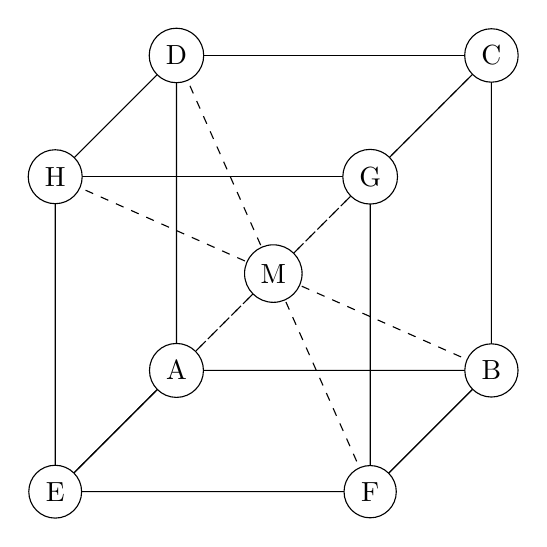
\begin{tikzpicture}[scale=2]
		\coordinate (a) at (0, 0, 0);
		\coordinate (b) at (2, 0, 0);
		\coordinate (c) at (2, 2, 0);
		\coordinate (d) at (0, 2, 0);
		\coordinate (e) at (0, 0, 2);
		\coordinate (f) at (2, 0, 2);
		\coordinate (g) at (2, 2, 2);
		\coordinate (h) at (0, 2, 2);
		\coordinate (m) at (1, 1, 1);

		\draw (a) -- (b) -- (c) -- (d) -- (a);
		\draw (e) -- (f) -- (g) -- (h) -- (e);
		\draw (a) -- (d) -- (h) -- (e) -- (a);
		\draw (b) -- (c) -- (g) -- (f) -- (b);
		\draw (a) -- (b) -- (f) -- (e) -- (a);

		\draw[dashed] (a) -- (m);
		\draw[dashed] (b) -- (m);
		\draw[dashed] (c) -- (m);
		\draw[dashed] (d) -- (m);
		\draw[dashed] (e) -- (m);
		\draw[dashed] (f) -- (m);
		\draw[dashed] (g) -- (m);
		\draw[dashed] (h) -- (m);

		\node[draw, circle, fill=white] at (a) {A};
		\node[draw, circle, fill=white] at (b) {B};
		\node[draw, circle, fill=white] at (c) {C};
		\node[draw, circle, fill=white] at (d) {D};
		\node[draw, circle, fill=white] at (e) {E};
		\node[draw, circle, fill=white] at (f) {F};
		\node[draw, circle, fill=white] at (g) {G};
		\node[draw, circle, fill=white] at (h) {H};
		\node[draw, circle, fill=white] at (m) {M};
	\end{tikzpicture}
	\caption{}
	\label{fig:}
\end{figure}

\fehlt

%%%%%%%%%%%%%%%%%%%%%%%%%%%%%%%%%%%%%%%%%%%%%%%%%%%%%%%%%%%%%%%%%%%%%%%%%%%%%%%
%                              Reziprokes Gitter                              %
%%%%%%%%%%%%%%%%%%%%%%%%%%%%%%%%%%%%%%%%%%%%%%%%%%%%%%%%%%%%%%%%%%%%%%%%%%%%%%%

\section{Reziprokes Gitter}
\label 3

\fehlt

%%%%%%%%%%%%%%%%%%%%%%%%%%%%%%%%%%%%%%%%%%%%%%%%%%%%%%%%%%%%%%%%%%%%%%%%%%%%%%%
%                     Bragg-Beugung und Röntgenstrahlung                     %
%%%%%%%%%%%%%%%%%%%%%%%%%%%%%%%%%%%%%%%%%%%%%%%%%%%%%%%%%%%%%%%%%%%%%%%%%%%%%%%

\section{Bragg-Beugung und Röntgenstrahlung}
\label 4

\fehlt

%%%%%%%%%%%%%%%%%%%%%%%%%%%%%%%%%%%%%%%%%%%%%%%%%%%%%%%%%%%%%%%%%%%%%%%%%%%%%%%
%                                    Ende                                     %
%%%%%%%%%%%%%%%%%%%%%%%%%%%%%%%%%%%%%%%%%%%%%%%%%%%%%%%%%%%%%%%%%%%%%%%%%%%%%%%

\IfFileExists{\bibliographyfile}{
	%\bibliography{\bibliographyfile}
}{}

\end{document}

% vim: spell spelllang=de
